
%\renewcommand\labelitemi{\textcolor{blue}{$\bullet$}}  
\renewcommand\normalcolor{\color{yellow}}  %for titles, etc.
\renewcommand\Black{\color{white}}        %for headers, etc.
\color{white}                             %for normal text


\foilhead{\textcolor{red}{C} Nebular Astrophysics}
\leftheader{C: Nebular Astrophysics}
\vpagecolor[blue]{RGBblack}                 %blue to black vertical gradient
\LogoOff
\bgclear

\vspace{-1cm}
\begin{center}
{\tt http://www.nublado.org/ }
\end{center}
\vspace{-1cm}
\begin{enumerate}
\item Atomic Processes.\\ 
Photoionization. Collisional Ionization. Recombination. Charge
Transfer. \label{item:processes}
\item Ionization Equilibrium. \\ 
Collisional Ionization in the low density limit. Photo-ionization
equilibrium.    \label{item:equi}
\item Thermal Balance.  \label{item:balance}
\item Nebular models. \\ CLOUDY. Analytical models:
pure hidrogen nebula, OTS approximation; dustry hydrogen nebula..
Problems with OTS - need for realistic radiative transfer. Escape
probabilities.  \label{item: models}
\item Temperature and density diagnostics. CELs, ORLs,
 Balmer \& Paschen discontinuities. The ORL/CEL discrepancy. \label{item: diag}
\item Detailed study: The Helix. \label{item:example}
\end{enumerate} 



\renewcommand\labelitemi{\textcolor{blue}{$\bullet$}}  
\renewcommand\normalcolor{\color{blue}}  %for titles, etc.

\foilhead{\textcolor{red}{C-\ref{item:processes}} Photoionization  }
\leftheader{C-\ref{item:processes}: Atomic processes}

\renewcommand\labelitemi{\textcolor{blue}{$\bullet$}}  
\renewcommand\Black{\color{black}}        %for headers, etc.
\renewcommand\labelitemii{\textcolor{DarkGreen}{$\star$}}  
\color{black}                             %for normal text

\LogoOff
\bgclear
\pagecolor{white}

In time-dependent perturbation theory, the rate of transition between
two states, $i\rightarrow f $, is:
\[
\frac{dP_{if}}{dt} = \frac{e^2}{h c^3 m_e^2} \sum_{\alpha = 1}^2 \int
\omega_{fi} ~\mathcal{N}_{\alpha}(\vec{k}) ~| \langle \phi_f |
e^{i\vec{k}\cdot\vec{x} } \vec{e}_{\alpha} \cdot \vec{p} | \phi_i
\rangle |^2 ~d\Omega,
\]   
where $\mathcal{N}(\vec{k})$ is the occupation number of photons in
the state corresponding to  $\vec{k}$,
with frequency  $\nu_{fi}$.

In a photoionization process the final states $f$ belong to the
continuum. The Born approximation neglects the influence of the ion on
$|\phi_f\rangle$, and for a description of the continuum we adopt a hard
box normalization, with a size  $L \rightarrow
\infty$. With  $i$ corresponding to the fundamental state of the
hidrogen atom, we obtain (Shu~I, 23),
\[
\frac{dP_{if}}{dt} \propto \omega_{fi}^{-3} \mathcal{N}(\omega),
~\text{where } \mathcal{N}(\omega) = \int d\Omega
\mathcal{N}(\vec{\omega}) .
\]

\end{document}

\foilhead{\textcolor{red}{C$_1$} Fotoionisaci\'on  }

La taza de absorpciones de fotones ionisantes con frecuencias en
$[\nu,\nu+\nu]$ es $ dN_f \frac{dP_{if}}{dt} $, en que $dN_f$ es el
n\'umero de estados libres en el rango correspondiente de
energ\'{\i}as,  
\[ 
dN_f = \frac{V}{2\pi^3} 4\pi~k_e^2 ~dk_e,
\]
en que $\vec{k_e}$ se refiere al electron libre.

La secci\'on eficaz de ionisaci\'on se define mediante
\[
P_{if} dN_f =  t~\sigma_{if}(\omega) c ~\frac{\mathcal{N}(\vec{n})}{V}
 ~4\pi n^2 dn , \text{~con } \frac{d^3\vec{n}}{V} =
\frac{d^3\omega}{(2\pi)^3 c^3}.
\]
Identificando para  $\sigma(\nu)$ se obtiene
\[
\sigma(\nu) \propto \nu^{-3}  g(\nu),
\]
donde $g(\nu)$ es un factor de gaunt, $g(\nu) \propto \nu^{-1/2} $ en
la aproximaci\'on de Born valida lejos del borde de ionisaci\'on
$\nu_\circ$. $g_\nu \approx 1 $ en la cercan\'{\i}a de $\nu_\circ$,
donde es mala la aproximaci\'on part\'{\i}cula libre. 


\foilhead{\textcolor{red}{C$_1$} Fotoionisaci\'on  }

\begin{center}
  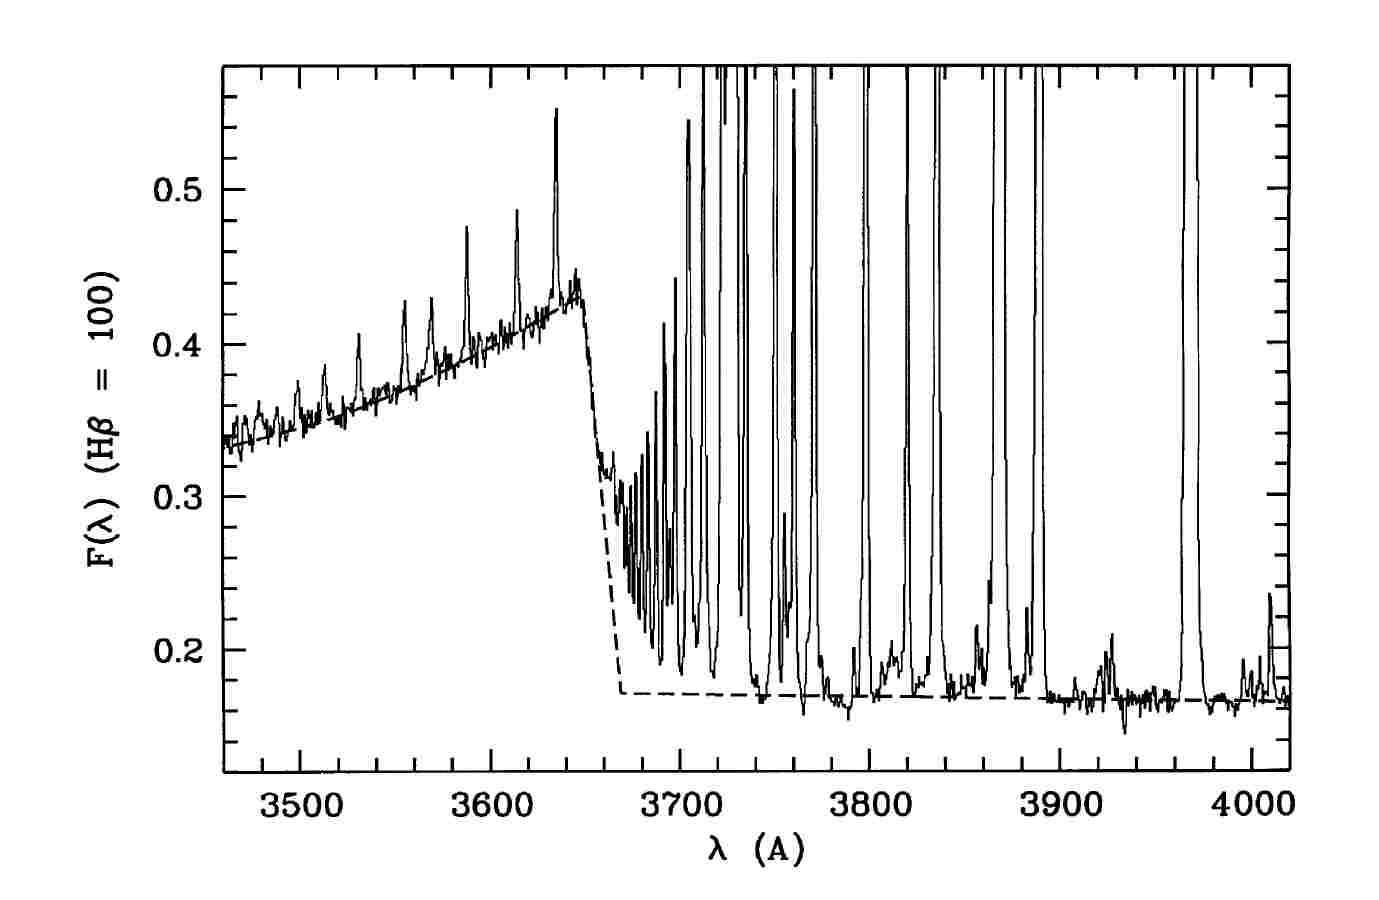
\includegraphics[width=25cm,height=!]{bj_liu.jpg}
\end{center}



\foilhead{\textcolor{red}{C$_1$} Fotoionisaci\'on de
  metales\footnote{Verner et al. 1996, ApJ, 465, 487. $1~b = 10^{-24}$~cm$^2$.}}


\begin{minipage}[t]{13cm}
  \begin{center}
    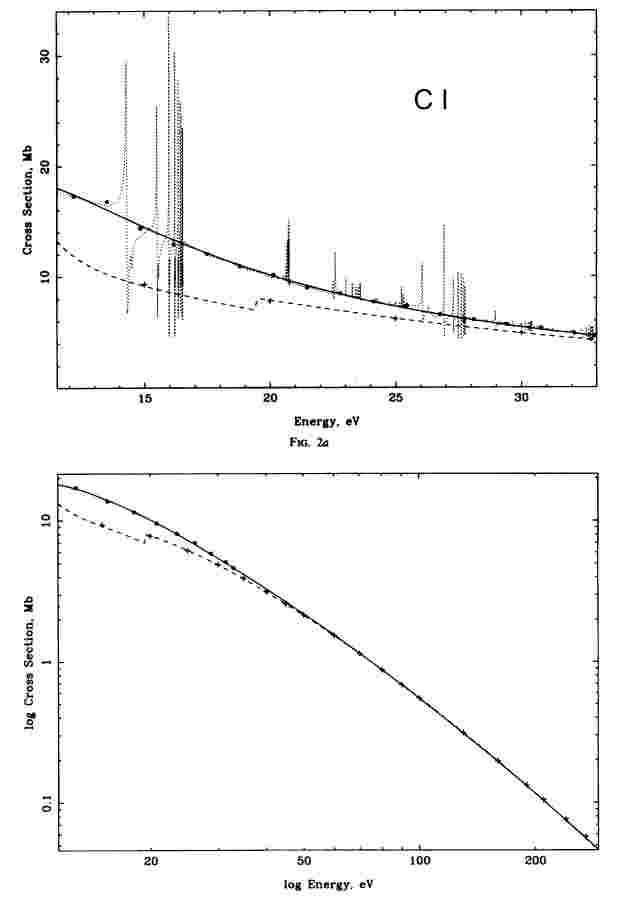
\includegraphics[width=12.5cm,height=16cm]{ci_photion.jpg}
  \end{center}
\end{minipage}
%\hfill
\begin{minipage}[t]{13cm}
  \begin{center}
    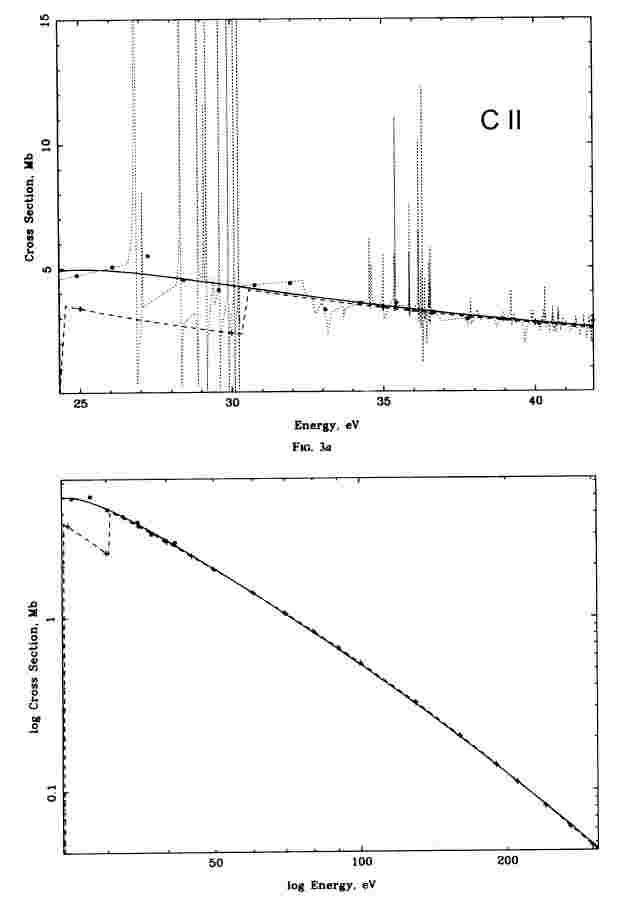
\includegraphics[width=12.5cm,height=16cm]{cii_photion.jpg}
  \end{center}
\end{minipage}

\foilhead{\textcolor{red}{C$_1$} Fotoionisaci\'on de
  metales\footnote{{\sc cloudy} manual, Hazy.}}

  \begin{center}
    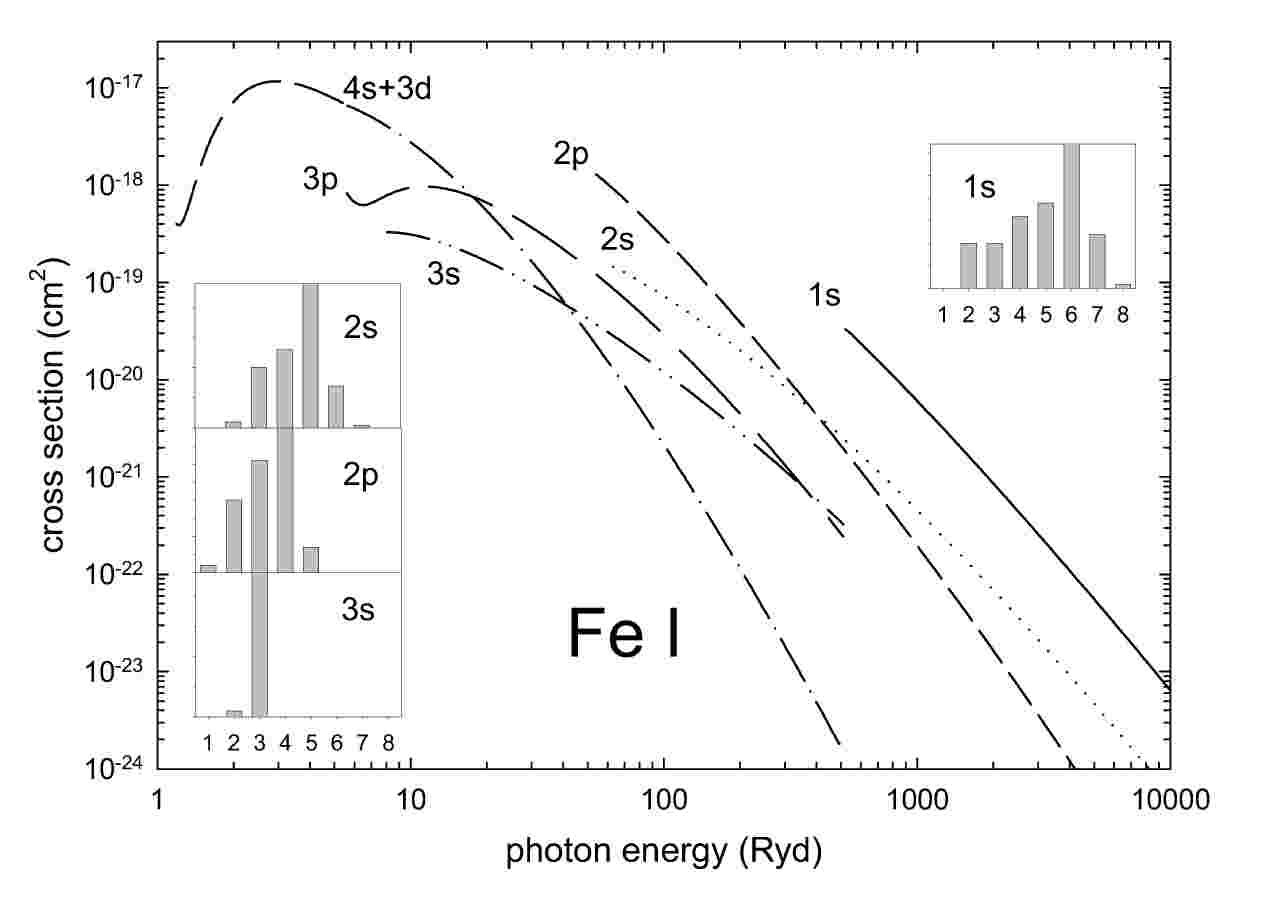
\includegraphics[width=!,height=16cm]{auger_FeI.jpg}
  \end{center}


\foilhead{\textcolor{red}{C$_1$} Ionisaci\'on colisional\footnote{Arnaud \& Rothenflug 1985, A\&AS, 60, 425, Arnaud \& Raymond, ApJ, 1992, 398, 394}}

\vspace{-2cm}
\begin{eqnarray}
\text{Ionisaci\'on colisional directa: }  & \mathrm{A} + \mathrm{e} \rightarrow \mathrm{A^+} + 2~\mathrm{e}   \nonumber \\ 
\text{Excitaci\'on  - auto-ionisaci\'on: }  & \mathrm{A} + \mathrm{e} \rightarrow \mathrm{A^\star} + \mathrm{e}   \nonumber  \\
                                         & \mathrm{A^{\star}}  \rightarrow \mathrm{A^+} + \mathrm{e}   \nonumber  
\end{eqnarray}
\vspace{-2cm}
\begin{center}
  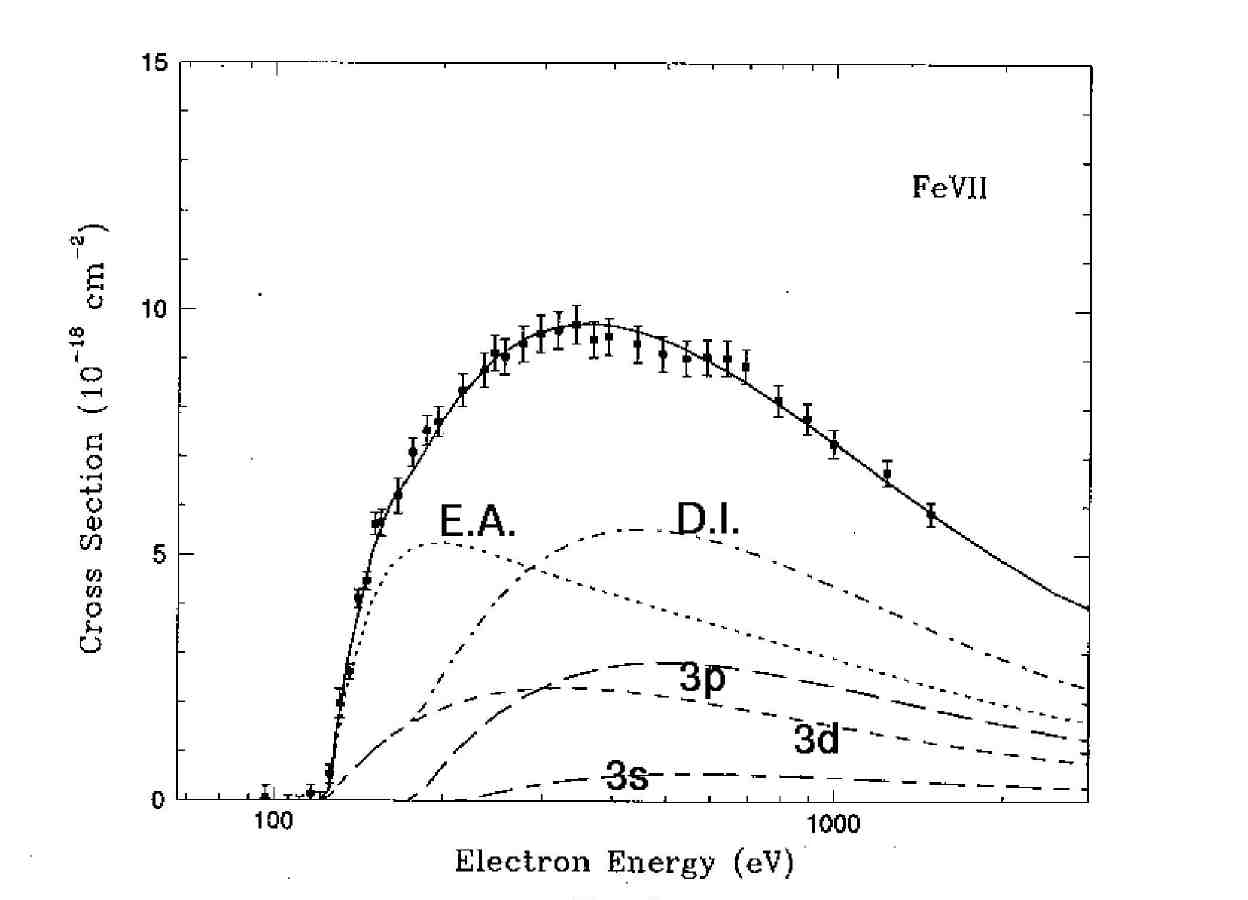
\includegraphics[width=17cm,height=!]{colion_xsec_2.jpg}
\end{center}


\foilhead{\textcolor{red}{C$_1$} Recombinac\'on}

{$\bullet$ Recombinac\'on radiativa} \\

La fotoionisaci\'on y su proceso inverso recombinaci\'on radiativa
estan relacionados por las relaciones de Einstein-Milne
(e.g. Osterbrock, A1; Shu I,75; Spitzer p104)).  El balance detallado
entre absorpciones de fotones con frecuencia $\nu$ y recombinaciones
de electrones e iones con velocidad relativa $v$ se escribe
\[
n_\mathrm{X} ~a_\nu 4 \pi \frac{B_\nu}{h \nu} ~d\nu = n_{\mathrm{X}^+} n_e
v \sigma(v) f(v) dv~ +~ n_{\mathrm{X}^+} n_e \sigma_2(v)  B_\nu v f(v) dv,
\]
con $~\frac{1}{2} m v^2 + h \nu_T = h \nu,$ y en que $f(v)$ es la
Maxwelliana integrada en \'angulo. Se obtiene (\textcolor{red}{tarea}) que  
$\sigma_2 = \sigma / (2 h \nu^3 / c^2 )$, y 
\[
\sigma(v) = \frac{g}{g_{+}}   \frac{h^2  \nu^2 }{m^2 c^2 v^2} a_\nu,    
\] 
 en que $g$ y $g_+$ son las degeneraciones de $X$ y $X^+$ en sus
 niveles fundamentales.


\foilhead{\textcolor{red}{C$_1$} Recombinac\'on}

{$\bullet$ Recombinac\'on colisional} \\

La recombinaci\'on a trav\'es de colisiones de 3 cuerpos 
\[
 \mathrm{A^+} + 2~\mathrm{e}  \rightarrow \mathrm{A} + \mathrm{e}, 
\]
importa en el l\'{\i}mite de muy altas densidades (que no es el
regimen de validez de los c\'alculos de equilibrio de ionisaci\'on
colisional, y que esta mejor descrito por la ley de masa-acci\'on), y
en el caso de la excitaci\'on de las l\'{\i}neas de recombinaci\'on
radio de H\,{\sc i} (por ejemplo H\,109$\alpha$ a 6\,cm, ver
Osterbrock p97).

\foilhead{\textcolor{red}{C$_1$} Recombinac\'on}

{$\bullet$ Recombinac\'on dielectr\'onica}

El proceso inverso de la excitaci\'on-autoionisaci\'on es la
recombinaci\'on dielectr\'onica. Por ejemplo (e.g. Osterbrock 1989) la
recombinaci\'on de C$^{++}$ en su configuraci\'on fundamental
$1s^22s^2~^1$S a trav\'es de una colisi\'on con un electron de
energ\'{\i}a 0.41~eV, que calza justo con la energ\'{\i}a de C$^+$ en
$1s^22p3d~^2$F. C$^{+}$ doblemente excitado decae despu\'es de una
cascada (en realidad 2 fotones, parando primero a $2s2p^2~^2$D) al nivel
fundamental $1s^22s^22p~^1$P$_{1/2}$.  Gen\'ericamente,
\[
\mathrm{X}^{+i+1} + e \rightarrow ~^{\star}\mathrm{X}^{+i} \rightarrow \mathrm{X}^{+i} + h\nu
\]
donde $^{\star}X^{+i}$ es un estado autoionisante de
$\mathrm{X}^{+i}$.  Este es el mecanismo dominate de recombinaci\'on a
temperaturas nebulares de $10^{4}$~K (Nussbaumer \& Storey, 1983,
A\&A, 126, 75). \underline{No se conoce para elementos mas pesados que
Ne}.

\foilhead{\textcolor{red}{C$_1$} Transfer de Carga}

(Spitzer + Osterbrock) 

\[
A  + H^+  \overset{k_1}{\underset{k_2}{\rightleftharpoons}} A^+ + H
\]
{$\bullet$ relaci\'on entre tazas de reacciones directa $k_1$ y reversa $k_2$}


\foilhead{\textcolor{red}{C$_2$} Equilibrio de ionisaci\'on}

{$\bullet$ Ionisaci\'on colisional}

En el l\'{\i}mite de bajas densidades, y sin fuente de ionisaci\'on
externa, las concentraciones relativas de los iones se obtienen del
balance detallado (el ejemplo es de Jordan (1969), pero son mejores
los n\'umeros de Arnaud et al.). 

\begin{center}
  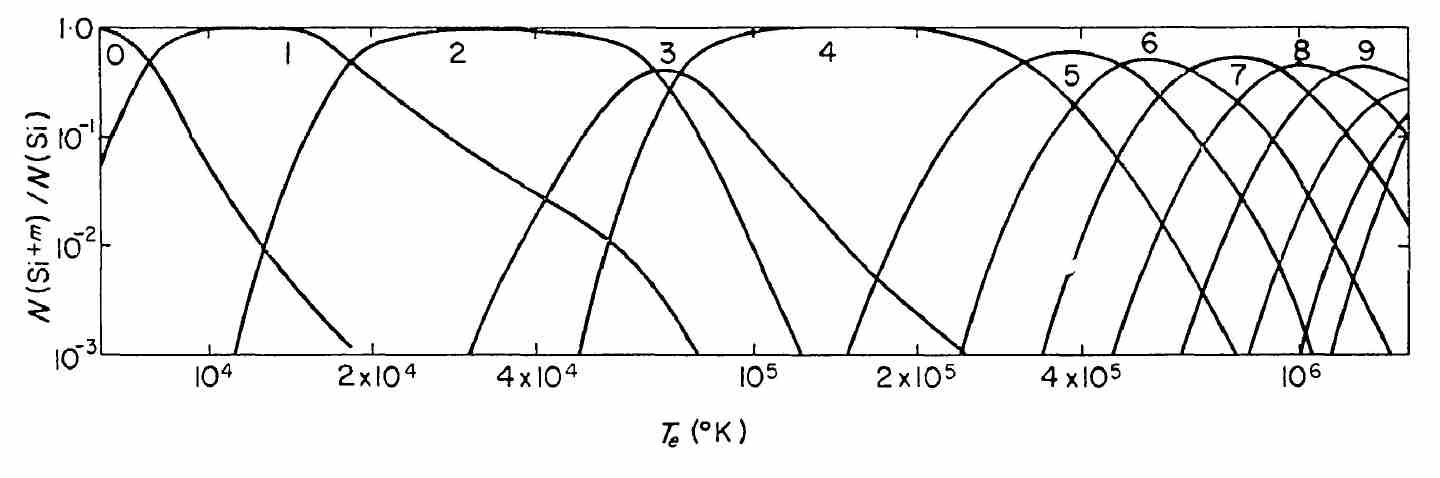
\includegraphics[width=25cm,height=!]{colion_eq.jpg}
\end{center}


\foilhead{\textcolor{red}{C$_2$} Equilibrio de ionisaci\'on - Fotoionisaci\'on}


La estructura de una nebulosa fotoionisada en simetr\'{\i}a esf\'erica
puede describirse por la fracci\'on de ionisaci\'on de cada elemento
en funci\'on del radio. Para un blob de material nebular, el balance
de ionisaci\'on requiere que el n\'umero de recombinaciones del ion
X$^{+i+1}$ sea igual al n\'umero de fotoionisaciones del ion X$^{+i}$,
\begin{equation}
N(\mathrm{X}^{i+1}) N_{e} \alpha_{T} = {\int}d{\nu} \frac{4\pi J_{\nu}}{h\nu}
a_{\nu} N(\mathrm{X}^{i}), 
\label{eq:ionisation_balance}
\end{equation}
en que $N_{e}$ es la densidad de electrones, $\alpha_{T}$ es el
coeficiente de recombinaci\'on total, y $a_{\nu}$ es la secci\'on
eficaz de fotoionisaci\'on, y $J_{\nu}$ es el promedio local en
\'angulos del campo nebular de intensidad espec\'{\i}fica, 
\begin{eqnarray}
J_{\nu}  & =  & \frac{1}{4~\pi}\int_{4 \pi} I_\nu d\Omega , \nonumber \\
 & = & \frac{1}{2}\int_{-1}^{+1} d\mu ~I_\nu(r,\mu), \text{~para
 simetr\'{\i}a  esf\'erica, con } \nonumber  \\ 
\mu &  =  & \cos \theta, \text{~en que $\theta$ es el \'angulo  con  el radio  vector.} \nonumber 
\end{eqnarray}


\foilhead{\textcolor{red}{C$_3$} Balance termal}

(R.E. Williams, en Lecture Notes on Introductory Theoretical
Physics). 

El ba\~no de electrones es la especie que m\'as r\'apida se termaliza
en una nebulosa ionisada (Spitzer, Cap. II). Consideramos el balance
energ\'etico de los electrones.

$\bullet$ {\bf \large calentamiento de los electrones}.
\begin{itemize}
\item des-excitaci\'on colisional. Importa en nebulosas densas, y es
 compensado parcialmente por excitaci\'ones colisionales.
\item fotoionisaci\'on. 
\end{itemize}

\foilhead{\textcolor{red}{C$_3$} Balance termal - fotoionisaci\'on}

Cada fotoelectr\'on entrega $\frac{1}{2} m v^2 = h \nu - I $ al ba\~no
de electrones, 
\[ 
G = N_\mathrm{H} \int_{\nu_1}^{\infty} 4 \pi J_\nu a_1(\nu) h (\nu -
\nu_1) d\nu  = N_\mathrm{H} \int_{\nu_1}^{\infty} 4 \pi J_\nu a_1(\nu) h (\langle
\nu \rangle  - \nu_1) d\nu,
\]
con 
\[
h\langle \nu \rangle = \int_{\nu_1}^{\infty} \frac{J_\nu}{h\nu}
a_1(\nu) h \nu d\nu  / \int_{\nu_1}^{\infty} \frac{J_\nu}{h\nu} a_1(\nu)  d\nu.
\]
En una buena aproximaci\'on $a_\nu = a_\circ (\nu_1/\nu)^3$, y en el
UV podemos usar el l\'{\i}mite de Wien para la radiaci\'on de cuerpo negro:
\[
J_\nu  \propto \nu^3 \exp(- \frac{h \nu} {k T_\star}. 
\]
\[\Rightarrow h \langle nu \rangle = \int_{\nu_1}^{\infty}
e^{-\frac{h\nu}{kT_\star}} / \int_{\nu_1}^{\infty} \frac{1}{\nu}
e^{-\frac{h\nu}{kT_\star}} d\nu = h\nu_1 + k T_\star. \]

\foilhead{\textcolor{red}{C$_3$} Balance termal - OTS}


En un estado estacionario, la ecuaci\'on de fotoionisaci\'on, $
\mathrm{H} + \nu \overset{k_1}{\underset{k_2}{\rightleftharpoons}}
\mathrm{H}^+ + \mathrm{e}^- , $ implica que $k_1 = k_2 $. En general
el campo de intensidad espec\'{\i}fica media $J_\nu(\vec{r})$ contiene
los fotones estelares, atenuados radialmente por absorpci\'on nebular,
y los fotones emitidos por la nebulosa.  La componente difusa es
compuesta en gran parte por fotones del cont\'{\i}nuo de Lyman, los
cuales pueden ser absorbido por hidr\'ogeno neutro en la nebulosa. En
la aproximaci\'on {\bf On-The-Spot} el equilibrio de ionisaci\'on $k_1
= k_2$,
\[
N(\mathrm{H\,{\sc i}})  \int_{\nu_1}^{\infty} d\nu  4 \pi J_\nu a_1(\nu)  / h
\nu = N_e N(\mathrm{H\,{\sc ii}}) \alpha, 
\]
en que $\alpha$ es el coeficiente de recombinaci\'on total, se puede
escribir
\[
N(\mathrm{H\,{\sc i}})  \int_{\nu_1}^{\infty} d\nu  4 \pi J^\star_\nu a_1(\nu)  / h
\nu = N_e N(\mathrm{H\,{\sc ii}}) \alpha^{(2)}, 
\]
en que $\alpha^{(2)} = \alpha - \alpha_1$.


\foilhead{\textcolor{red}{C$_3$} Balance termal - calentamento neto}


 La secci\'on eficaz de
recombinaci\'on radiativa tiene la forma t\'{\i}pica de
interacci\'ones Coulombianas, $\propto 1/v^2$, 
\[
\sigma_\mathrm{rec} = \sigma_\circ (v_\circ/v)^2, 
\]
lo cual sale de la relaci\'on de Milne $\sigma_\mathrm{rec}(v) = \nu^2
a_\nu / v^2.$ Promediando en velocidades, 
\[
\alpha^{(2)} =  \langle v \sigma_\mathrm{rec} \rangle \propto
\langle  \frac{1}{v}   \rangle \propto 1/\sqrt{T_e}.
\]

\foilhead{\textcolor{red}{C$_3$} Balance termal - enfr\'{\i}amento}

$\bullet$ {\bf \large Enfr\'{\i}amento de los  electrones}.

\begin{itemize}
\item Excitaci\'on colisional.
\item Recombinaciones.
\end{itemize}

\underline{\bf Nebulosa de hidr\'ogeno puro}\\

Los niveles excitados de H estan a energ\'{\i}as inalcansables para
temperaturas t\'{\i}picas de nebulosas fotoionisadas, 13.6~(1-1/4)~eV
corresponde a $T\approx 10^5~$K. $\Rightarrow$ domina el
enfr\'{\i}amento por recombinaciones, o sea \[ L_R = N_e N(\mathrm{H\,{\sc
ii}}) \alpha^{(2)} \frac{1}{2} m \langle v^2 \rangle \propto
\sqrt{T_e}.
\]
$\Rightarrow$ Para una nebulosa de hidr\'ogeno puro, $T_e = \frac{2}{3}
k T_\star$. 


\foilhead{\textcolor{red}{C$_3$} Balance termal - enfr\'{\i}amento por
metales}


\underline{\bf Nebulosa con metales}\\

La excitaci\'on colisional de los niveles de estructura fina (y
tambi\'en con $\Delta L$) de los iones pesados, como S, N, O, C, estan
s\'olo a $\chi \lesssim 3$~eV. Excitaci\'on colisional seguida por
des-excitaci\'on radiativa es el principal mecanismo de
enfr\'{\i}amento de nebulosas foto-ionisadas:
\[
L_C = N_e N(X^i) \langle \sigma_e v \rangle  \chi, 
\]
con
\[
\langle \sigma_e v \rangle  =  \frac{1}{\sqrt{T_e}} \exp( - \frac{\chi}{kT_e}). 
\]



\foilhead{\textcolor{red}{C$_4$} Modelos de nebulosas}

La razon de abundancias i\'onicas en estados de ionisaci\'on
consecutivos,
$Q_{\mathrm{X}^{i}}=N(\mathrm{X}^{i+1})/N(\mathrm{X}^{i})$, se obtiene
facilmente del equilibrio de ionisaci\'on
(Eq.~\ref{eq:ionisation_balance}) si el campo ionisante es conocido. 
  

%Note that if the ionising potential of X$^{+i}$ is higher than the
%second ionisation energy of helium, $h\nu > 54 eV$, and if the nebula
%is optically thin at $\nu$, a guess at the outer radius of the nebula
%allows an estimate of the volume average of $Q_{X^{i}}$. Unfortunately
%what is observable is the ratio of the volume averages of the ionic
%abundances.

Dado un campo de densidad $N_e$ y temperatura $T_e$, la estructura de
una nebulosa fotoionisada se calcula num\'ericamente avanzando en
radio. Este es el principio fundamental del c\'odigo de
fotoionisaci\'on {\small CLOUDY}, por Gary Ferland et al.. La
comparaci\'on de flujos modelos con l\'{\i}neas i\'onicas observadas
debiera ser una buena herramienta para estudiar las condiciones
f\'{\i}sicas en las nubes. Pero las bases de datos at\'omicos son
aproximadas, y las incertezas en los coeficientes de rec. diel. se
propagan desde los primeros estados de ionisaci\'on. \\


\foilhead{\textcolor{red}{C$_4$} Modelos de nebulosas}


\bgaddcenter{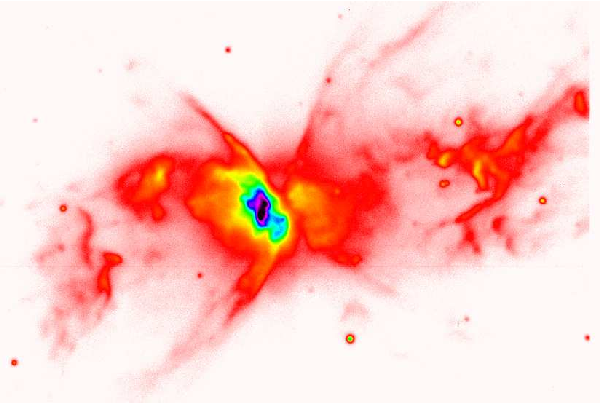
\includegraphics[width=!,height=\textheight]{ngc6302_Rband.pdf}}
\vspace{5cm}
\begin{center}
  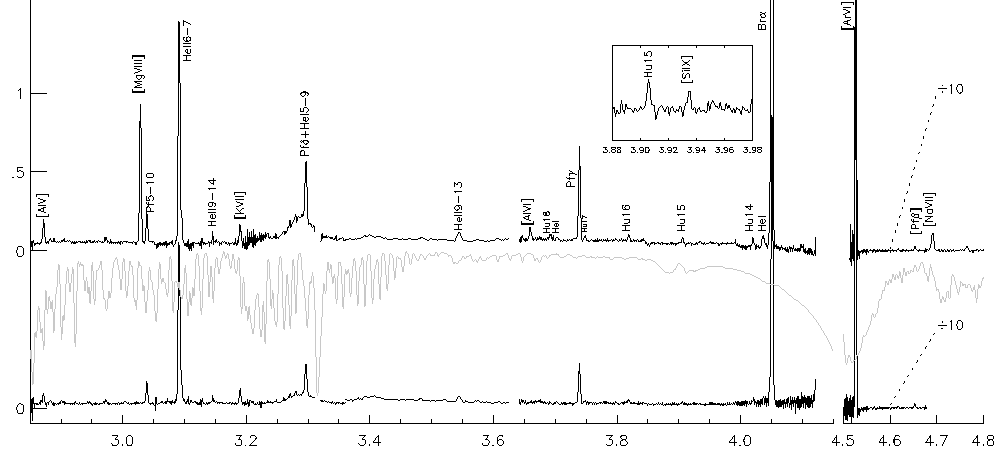
\includegraphics[width=25cm,height=!]{specCGS4.pdf}
\end{center}


\foilhead{\textcolor{red}{C$_4$} Modelos de nebulosas}

\vspace{4cm}
\begin{center}
  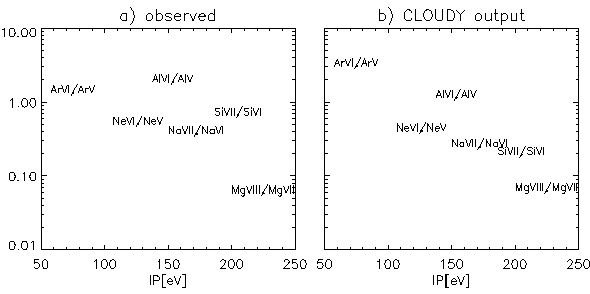
\includegraphics[width=25cm,height=!]{ioncurve.pdf}
\end{center}

\foilhead{\textcolor{red}{C$_4$} Modelos de nebulosas}

\vspace{10cm}
\begin{center}
  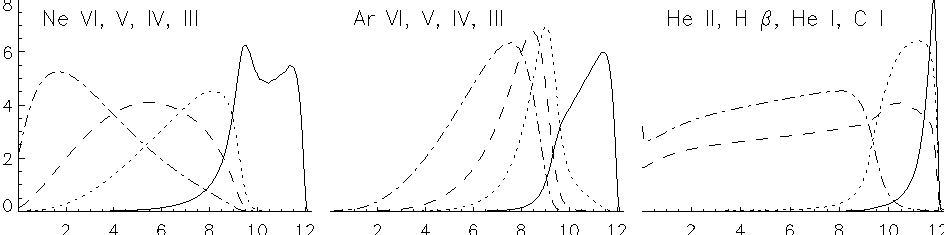
\includegraphics[width=25cm,height=!]{struct_n6302.pdf}
\end{center}




\foilhead{\textcolor{red}{C$_4$} Modelos de nebulosas}

\bgclear

Ejemplo de input para CLOUDY: {\tt parispn.in}\\

\medskip
\medskip
\medskip

{\tt black body, T=150,000K radius = 10\\
hden = 3.4771213\\
radius = 17\\
normalize to   Ca b  ~ 4861\\
abund he -1 C-3.523 N-4. O-3.222 ne-3.824 mg-4.523\\ 
}

\medskip

\textcolor{red}{Tarea}: Correr el modelo de validaci\'on de CLOUDY 96
{\tt parispn.in}, y graficar la fraction relativa de cada i\'on de Ne
en funci\'on del radio.




\foilhead{\textcolor{red}{C$_4$} Modelos de nebulosas}

{$\bullet$ Esf\'eras de Str\"omgren}

{$\bullet$ Nebulosa de hidr\'ogeno puro}

\textcolor{red}{Tarea}: Problema 3-1 de Shu I. 

{$\bullet$ Nebulosa de regi\'on H\,{\sc ii} de hidr\'ogeno puro + polvo}

(Petrosian, Silk \& Field, 1972, ApJ, 177, 69; Spitzer)

{$\bullet$ Discusi\'on de la aproximaci\'on OTS}.

ver {\tt dhii.pdf}. 


\foilhead{\textcolor{red}{C$_5$} Diagn\'osticos de composici\'on,
temperatura y densidad }

{$\bullet$ \bf L\'{\i}neas de recombinaci\'on de H\,{\sc i}, He\,{\sc
ii}, y He\,{\sc i} } \\

El flujo de una l\'{\i}nea de hidr\'ogeno en el \'optico es $F_{ij} =
\int ds d\Omega j_{ij}$, donde la emisividad de una transici\'on $n_i
\leftarrow n_j$ poblada por la cascada de recombinaci\'on es
\[ 
j_{ij} = \frac{h  \nu}{4 \pi} \sum_{L_i=0}^{n-1} \sum_{L_j=L_i\pm1}
N_n h\nu_{ij}
\]
Los n\'umeros de ocupaci\'on $N_n$ se puede calcular
teor\'{\i}camente, y son una funci\'on debil de ${T_e,N_e}$. Para
calcularlos se da cuenta de los efectos de transfer con una
aproximaci\'on OTS que distingue dos casos (Baker \& Menzel 1938, ApJ,
88, 52): caso A, donde la nebulosa es \'opticamente delgada en todas
las transiciones (y tambi\'en en el continuo de Lyman), y caso B en
que todos los fotones de la serie de Lyman, y del cont\'{\i}nuo de
Lyman, son absorbidos OTS, de manera que el nivel fundamental efectivo
en el c\'alculo es $n=2$.

\foilhead{\textcolor{red}{C$_5$} L\'{\i}neas de recombinaci\'on}

Se define el coeficiente de recombinaci\'on efectivo con
\[
N_p N_e \alpha_{ij}^\mathrm{eff} = \frac{4 \pi}{h \nu_{ij}}  j_{ij}.
\]
Hummer \& Storey (1987, MNRAS, 224, 801) dan
$\alpha_\mathrm{H\beta}^\mathrm{eff} =3.0~10^{-14}~$cm$^{-3}$, a
$10^4$~K (aprox.  $\propto
\sqrt{1/T_e}$), y tabulan las emisividades  de  las l\'{\i}neas de
recombinaci\'on relativas a $H_\beta$ para H\,{\sc i} y H\,{\sc
ii}. Las transiciones de He\,{\sc i} estan tabuladas por Smits, MNRAS,
251, 316. Las de O\,{\sc ii}, N\,{\sc ii}, N\,{\sc iii}, Ne\,{\sc ii},
C\,{\sc ii} y C\,{\sc iii} tambi\'en se encuentran en referencias
recientes. 

Notar que con el flujo de una l\'{\i}nea de recombinaci\'on y la
densidad $N_e$ es directo obtener la columna del ion
correspondiente. Por ejemplo el espectro de recombinaci\'on de O\,{\sc
ii} da la columna de O$^{2+}$, que tiene el espectro O\,{\sc iii}.

\foilhead{\textcolor{red}{C$_5$} L\'{\i}neas excitadas por colisiones - CELs.}


Una predicci\'on para el flujo de una CEL $i \leftarrow j$ \'optica
delgada se obtiene integrando su emisividad en el camino \'optico $s$:
\[
I_{ij} = \int ds \, d\Omega ~ j_\nu = \int ds \, d\Omega ~ \frac{b\,
A_{ij}\, h\nu_{ij}}{4\pi}~ N_j ,
\]
en que $N_j$ es la poblaci\'on en el nivel excitado $j$, y donde $b$
es el `branching ratio', que permite considerar el caso general cuando
nacen m\'as de una transici\'on de un mismo nivel con tasa de
decaimento espont\'aneo $A_{ij}$. \\


El diagn\'ostico de las condiciones f\'{\i}sica en una nebulosa
ionisada en base a l\'{\i}neas de emisi\'on radica entonces en la
dependencia de $N_j(\vec{r})$ en $T_e,N_e$. Despreciando transiciones
radiativas y recombinaci\'on,
\[
\sum_{i{\neq}j}
{n}_{j}{C}_{ji} +
\sum_{i<j}{n}_{j}{A}_{ji} = \sum_{i{\neq}j}{n}_{i}{C}_{ij}  + \sum_{i>j}{n}_{i}{A}_{ij}, 
\]
donde $N_j = n_j \, N_\circ$, y $N_\circ$ es la densidad de iones en
el nivel fundamental. En acoplamiento LS las reglas de Hund dan 2 a 5
niveles en la configuraci\'on fundamental para iones de interes.

\foilhead{\textcolor{red}{C$_5$} Diagn\'osticos de composici\'on,
temperatura y densidad }

{$\bullet$} Pares de l\'{\i}neas sensibles a la densidad.  \\

%\begin{minipage}[t]{11cm}
%  \begin{center}
%    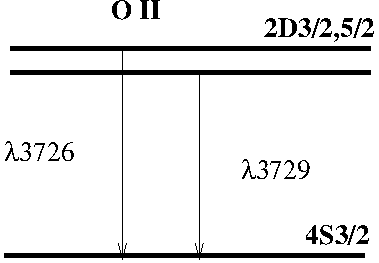
\includegraphics[width=10cm,height=!]{oii.pdf}
%  \end{center}
%\end{minipage}
%%\hfill
%\begin{minipage}[t]{15cm}

\begin{floatingfigure}{12cm}
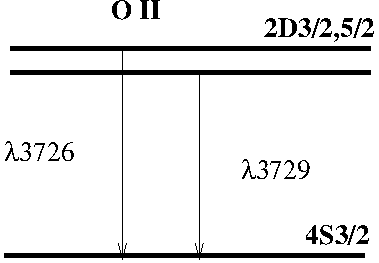
\includegraphics[width=9cm,height=!]{oii.pdf}
\end{floatingfigure}  \quad  Las densidades cr\'{\i}ticas de ambas
l\'{\i}neas son $N_c(\lambda3729) = 4\,10^{13}$cm$^{3}$ y
$N_c(\lambda3726) = 2\,10^{4}$cm$^{-3}$, ambas comparables con
densidades t\'{\i}picas de nebulosas. La raz\'on de estas l\'{\i}neas
no depende de la concentraci\'on de O$^+$.  Como los niveles
superiores estan muy cercanos en energ\'{\i}as, sus poblaciones son
insensibles a la temperatura. El doblete de [O\,{\sc ii}] es un buen
indicador de densidad cuando esta es cercana a las densidades
cr\'{\i}ticas. Consideramos la razon de intensidades de estas dos
l\'{\i}neas en regimenes de densidad t\'{\i}picos.

\foilhead{\textcolor{red}{C$_5$} Diagn\'osticos de composici\'on,
temperatura y densidad }


\begin{itemize}
\item $N_e \ll N_c$. \[ \frac{I(\lambda 3279)}{I(\lambda 3726)} =\frac{ N_e
N_1  \langle \sigma_{12} \rangle \frac{h\nu_{21}}{4\pi}}{ N_e
N_1  \langle \sigma_{13} \rangle \frac{h\nu_{31}}{4\pi}} = \frac{ \langle
\sigma_{12} v  \rangle}{\langle \sigma_{13} v  \rangle},\] independiente de
$N_e$\footnote{y de $T_e$ porque $\sigma  \propto g$ para niveles de
estructura fina} 
\item $N_e \gg N_c$. En este caso $N_3 = N_1 C_{13}/C_{31} = N_1 g_3
e^{-\chi_3/kT} / g_1 $  y 
\[\frac{I(\lambda 3279)}{I(\lambda 3726)} = \frac{A_{21}
N_2 g_2 }{A_{31}N_3 g_3}, \] independiente de $N_e$ y muy debilmente
en $T_e$.
\item En el caso intermediario, consideremos $N_c(\lambda 3729) \ll N_c
\ll N_c(\lambda 3726)$:
\[\frac{I(\lambda 3279)}{I(\lambda 3726)} = \frac{g_2}{g_3}
\frac{A_{21}}{N_e \langle \sigma_{12} v \rangle} \propto \sqrt{T_e}/N_e,\]  una funci\'on de
$N_e$.
\end{itemize}

%\end{minipage}



\foilhead{\textcolor{red}{C$_5$} Pares de l\'{\i}neas sensibles a la temperatura.}  

%\begin{minipage}[t]{8cm}
%  \begin{center}
%    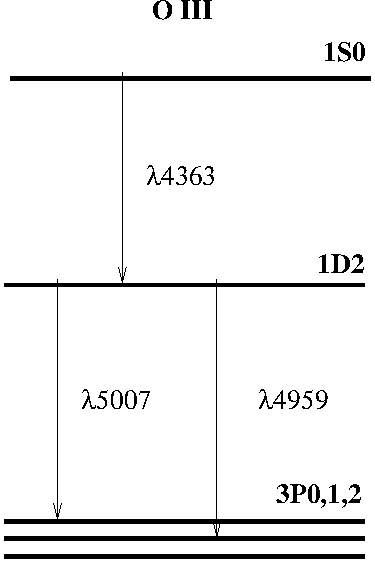
\includegraphics[width=7cm,height=!]{oiii.pdf}
%  \end{center}
%\end{minipage}
%    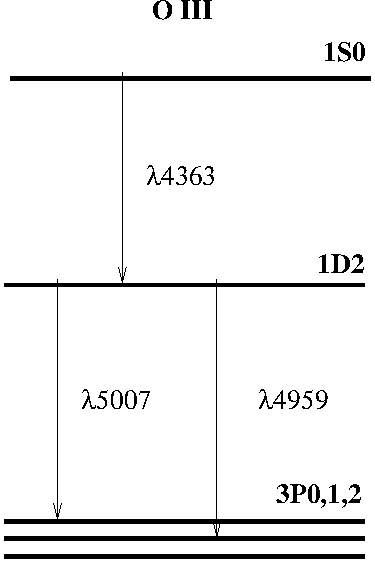
\includegraphics[width=7cm,height=!]{oiii.pdf}
%\hfill
%\begin{minipage}[t]{15cm} 
%\vspace{-8cm}
\begin{floatingfigure}{8cm}
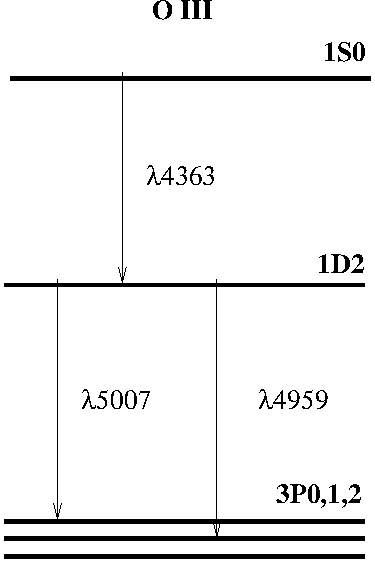
\includegraphics[width=7cm,height=!]{oiii.pdf}
\end{floatingfigure}  Estas tres transiciones tienen $A \gtrsim 1$~s$^{-1}$, y $N_c \gg
10^{4}$~cm$^{-3}$, y $A_{32} \ll A_{31}$, de manera que
\begin{eqnarray}
j(\lambda4363) & = &  N_e N_1 \langle \sigma_{13} v \rangle \frac{h \nu_{32}}{4\pi}, \nonumber \\
j(\lambda5007) & = &  N_e N_1 \left[ \langle \sigma_{12} v \rangle  +
\langle \sigma_{13} v \rangle  \frac{A_{32}}{A_{31}+A_{21}} \right] \frac{h \nu_{21}}{4\pi}, \nonumber 
\end{eqnarray}
en que hemos tratado $\lambda4959$ y $\lambda5007$ como una sola
l\'{\i}nea. La raz\'on de estas {\bf dos} l\'{\i}nas es 
\[
\frac{I(\lambda 5007)}{I(\lambda4363)} = \frac{\lambda_{32}}{\lambda_{21}}
\left[1+\frac{\langle \sigma_{12} v \rangle}{\langle \sigma_{13} v
\rangle } \right].
\]
Recordando que $\langle \sigma_{ij} v \rangle \propto T_e^{-1/2}
e^{-\chi_{ij}/kT_e}$, vemos que la razon $\frac{I(\lambda
5007)}{I(\lambda4363)} $ es sensible a la temperatura. Se obtiene
$\frac{I(\lambda 5007)}{I(\lambda4363)} \approx 8~\exp(33000/T_e)$.

%\end{minipage}



\foilhead{\textcolor{red}{C$_5$}  L\'{\i}neas de recombinaci\'on  y densidad }


\begin{floatingfigure}{14cm}
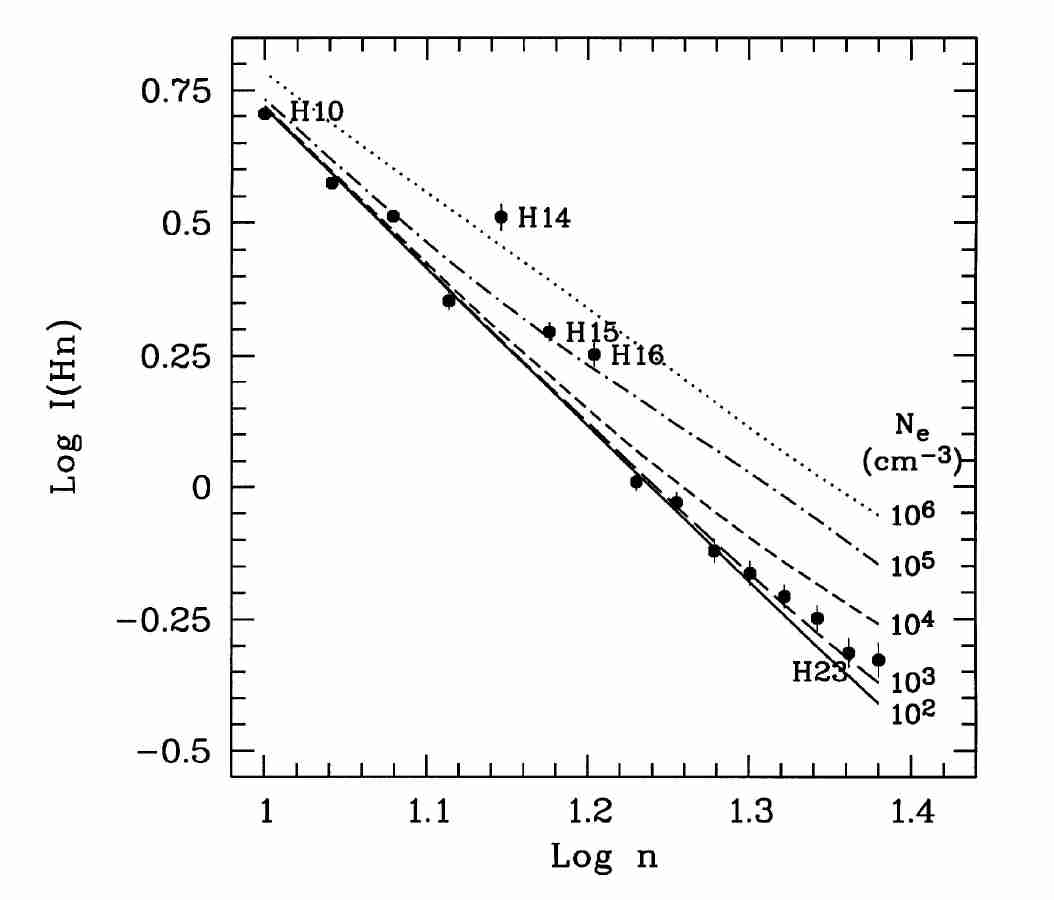
\includegraphics[width=13cm,height=!]{Hn_Ne.jpg}
\end{floatingfigure}  Las l\'{\i}neas de recombinaci\'on tienene una
leve dependencia en la densidad que se puede usar como diagn\'ostico
(Liu et al. 2000, MNRAS, 312, 585). 

\foilhead{\textcolor{red}{C$_5$} Relaci\'on l\'{\i}nea-cont\'{\i}nuo-temperatura.   }

La densidad de flujo en el cont\'{\i}nuo libre-libre a radio
frecuencias se relaciona con el flujo de H$\beta$ con
\[
F(H\beta) = 0.28 T_e^{-0.52} \nu^{0.1} F_\nu,
\]
de lo cual podemos despejar $T_e$. Las l\'{\i}neas de recombinaci\'on
a $n\gg 1$ en ondas radios tienen la ventaja de no depender de la
extincci\'on, y sus emisividades se calculan en LTE (la correcci\'on
es $\ll 1$ y esta tabulada por Brocklehurst (1970, MNRAS 148, 417).


\foilhead{\textcolor{red}{C$_5$} Discontinuidades de Balmer y Paschen.   }

\begin{minipage}[t]{13cm}
$BJ = \frac{I_c(\lambda3643)-I_c(\lambda3681)}{I(H11,\lambda3770)}.$ \\
$I_c(\lambda)$ esta tabulada por Brown \& Mathews (1970, ApJ, 160,
939).

\begin{center}
  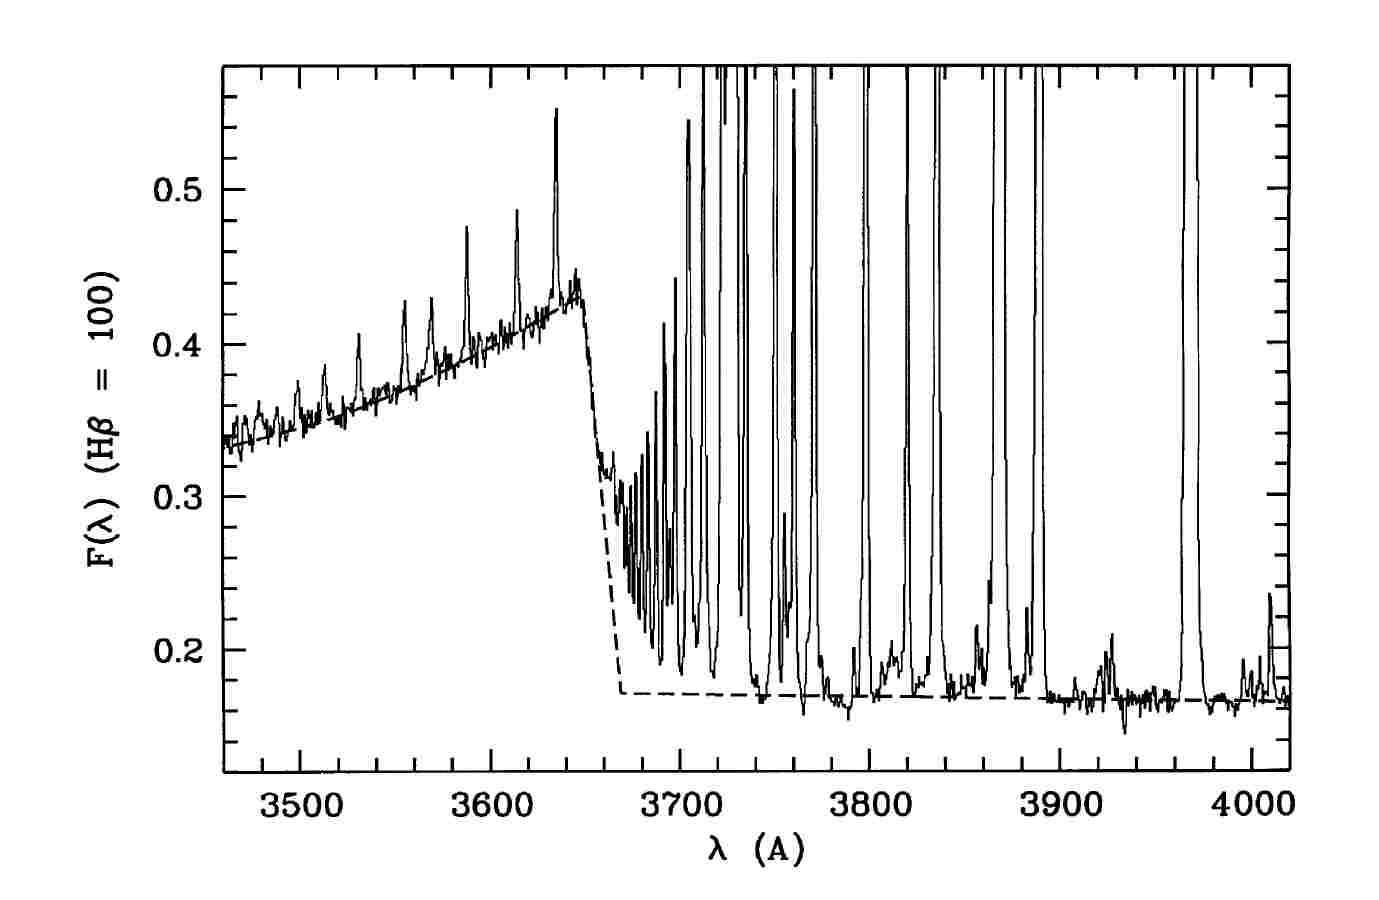
\includegraphics[width=12.5cm,height=!]{bj_liu.jpg} \end{center}
\end{minipage}
\hfill
\begin{minipage}[t]{13cm}
He$^+$/H$^+$ = 0.1, He$^{++}$/H$^+$=0 (dots);
He$^+$/H$^+$ = He$^{++}$/H$^+$=0.05   (solid);
He$^+$/H$^+$ = 0, He$^{++}$/H$^+$=0.1   (dashed).
  \begin{center}
    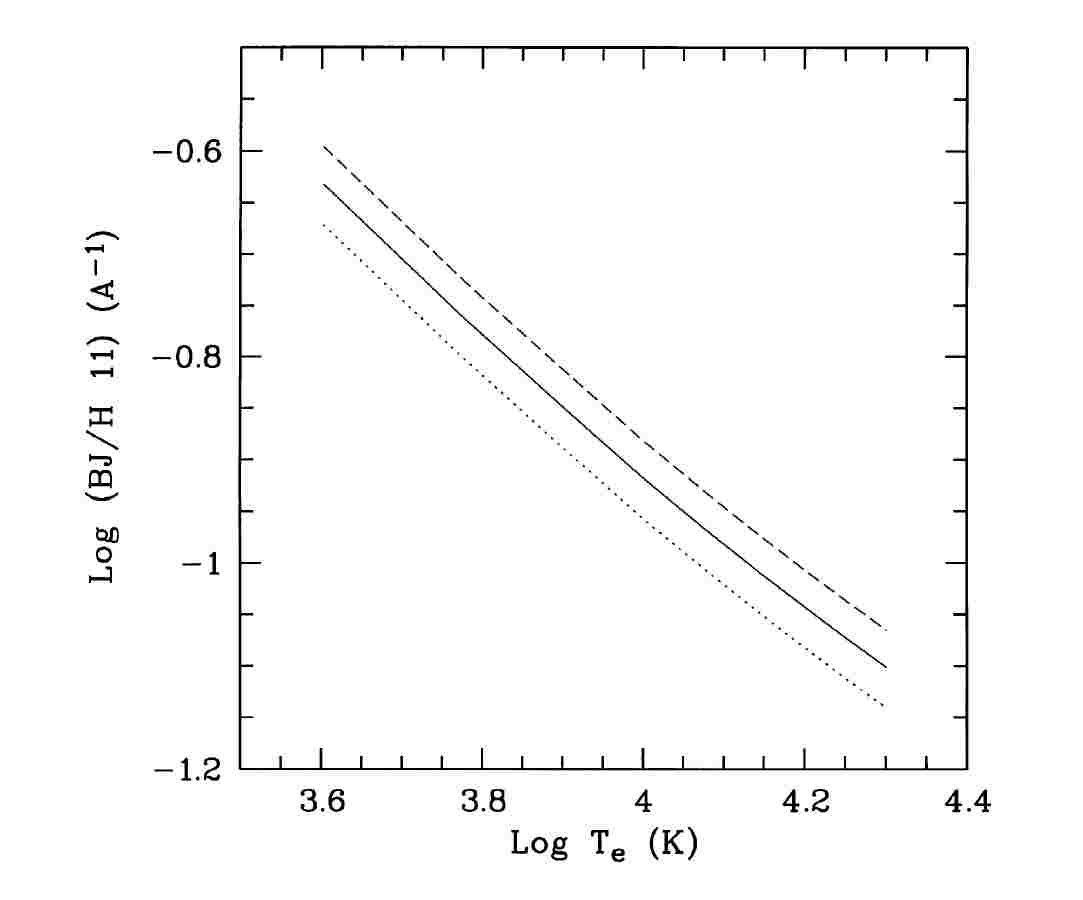
\includegraphics[width=12.5cm,height=!]{BJ_T.jpg}
  \end{center}
\end{minipage}

El mismo an\'alisis se puede hacer con la discontinuidad de Paschen a
8194\AA.


\foilhead{\textcolor{red}{C$_5$} La discrepancia ORL/CEL.  }

\begin{center}
      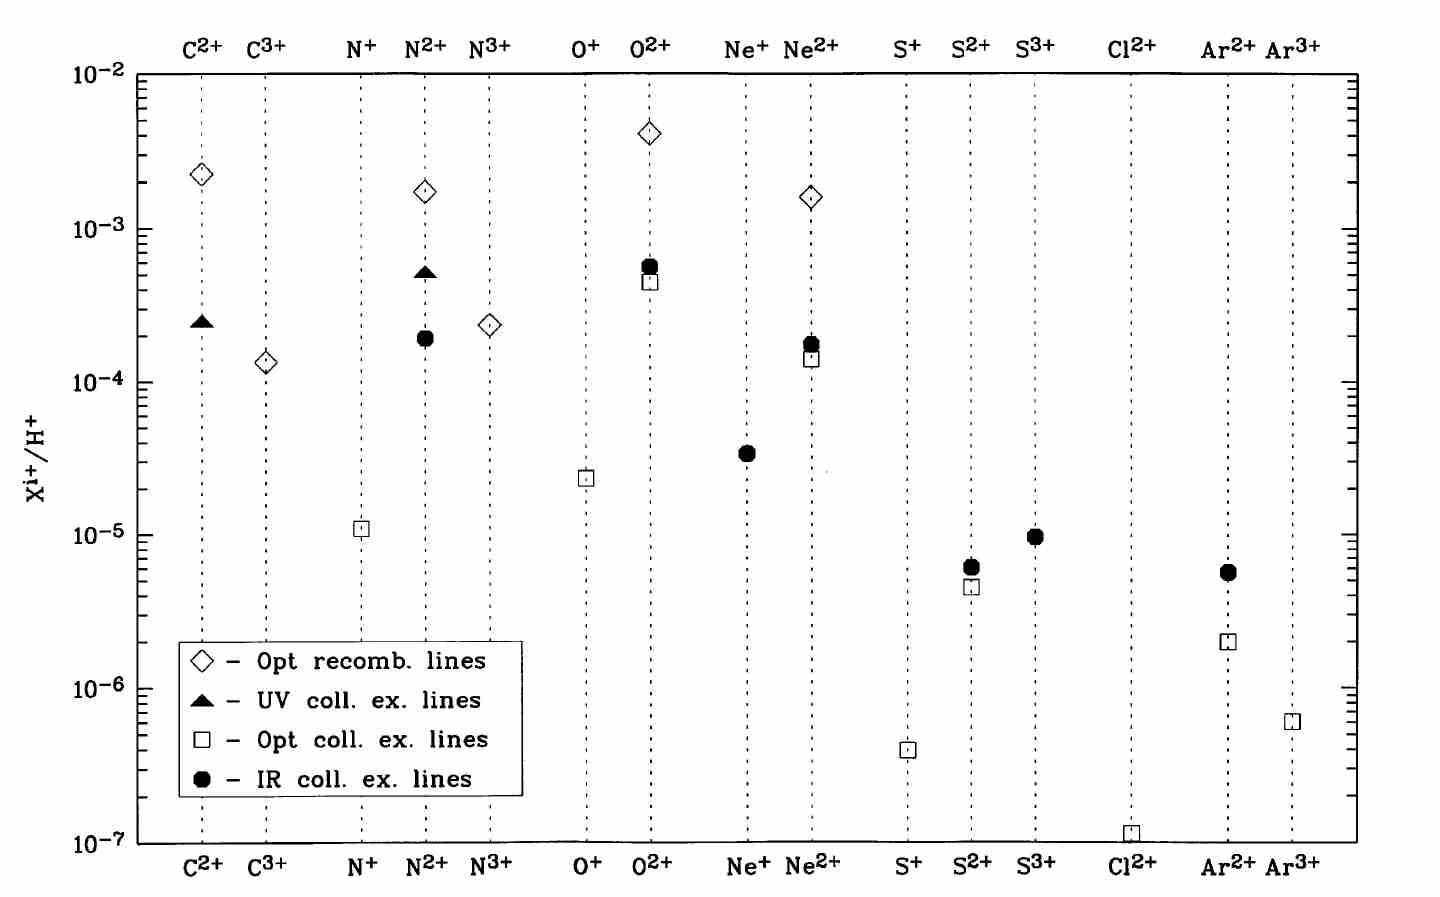
\includegraphics[width=0.9\textwidth,height=!]{ORL_CEL_general.jpg}
\end{center}


\foilhead{\textcolor{red}{C$_5$} La discrepancia ORL/CEL.  }

\begin{itemize}
\item En principio los mejores indicadores de abundancias i\'onicas son las
ORLs, porque los coeficientes de recombinaci\'on efectivos de los
iones y de hidr\'ogeno tienen son approx. $\propto 1/\sqrt{T_e}$, y la
dependia resiudal en temperatura es muy debil. 

\item El problema con las ORLs es que sus flujos son $10^{-3} --
10^{-4}$ los de H$\beta$.

\item En contraste las CELs tienen una dependencia exponencial en la
temperatura, y sus flujos son comparables a H$\beta$. 

\end{itemize}

\foilhead{\textcolor{red}{C$_5$} La discrepancia ORL/CEL.  }

\begin{center}
      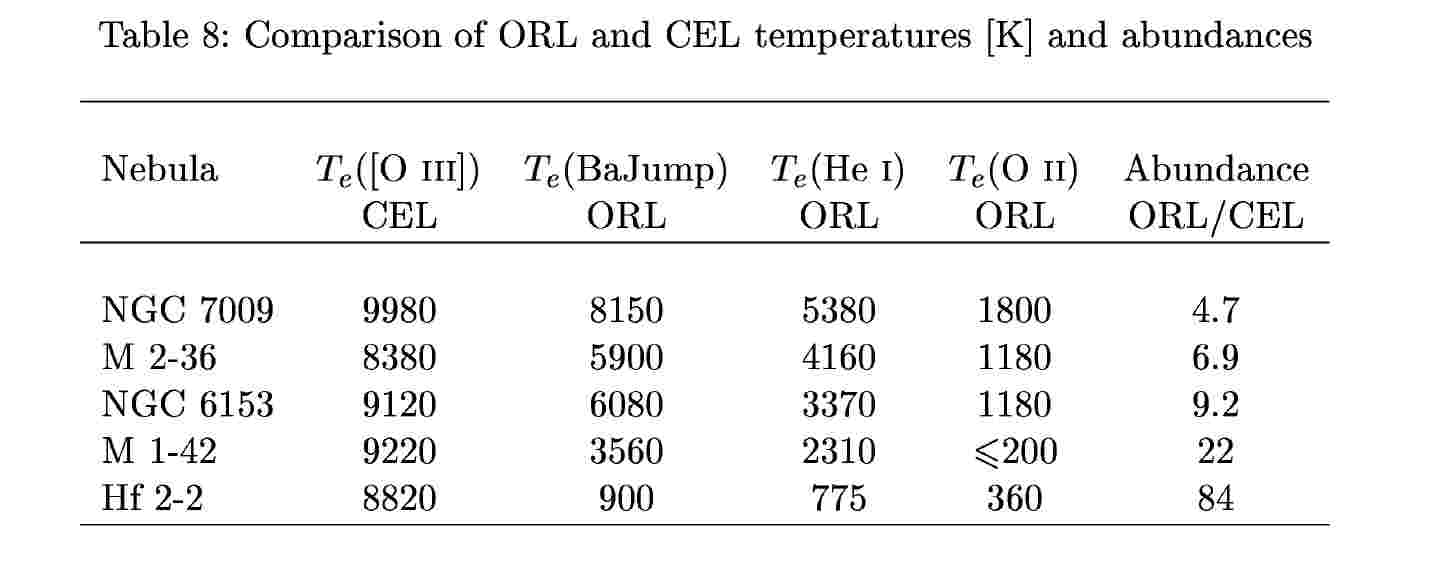
\includegraphics[width=\textwidth,height=!]{orl_cel_table.jpg}
\end{center}

Se observa una discrepancia sistema entre las CELs y las ORLs: 
\begin{itemize}
\item $T_e(\mathrm{CEL}) > T_e(\mathrm{ORL} \sim T_e(\mathrm{continuo})$
 
\item $N(X^{+i})(\mathrm{CEL}) < N(X^{+i})(\mathrm{ORL})$.  Pero las
columnas son iguales al usar las mismas temperaturas. 
\end{itemize}


\foilhead{\textcolor{red}{C$_5$} La discrepancia ORL/CEL -
fluctuaciones de temperatura.  }

Una estrategia para reconciliar la discrepancia en temperatura,
propuesto originalmente por Peimbert (1967, ApJ, 150, 825) para
explicar la sistem\'atica discrepancia entre $T($O\,{\sc iii}) y
$T(\mathrm{continuo})$, es el formalismo ``$t^2$''. En este formalismo
se introducen peque\~nas fluctuaciones de temperatura en torno a un
valor medio ponderado por la medida de emisi\'on del i\'on en
cuesti\'on:
\[
j(T) = j(T_\circ) + (T-T_\circ)
\left. \frac{dj}{dT}\right|_{T=T_\circ} + \left. \frac{1}{2} (T-T_\circ)^2
\frac{d^2j}{dT^2}\right|_{T=T_\circ}, \text{y integrando en ds,}
\]
\[
\int N_e N_i j(T) ds = j(T\circ) \int N_i N_e ds + \left. \frac{1}{2}
\frac{d^2j}{dT^2}\right|_{T=T_\circ} \int ds N_i N_e (T-T_\circ)^2,
\]
en que el t\'ermino de orden 1 se cancela al elegir 
\[
T_\circ = \int ds N_i N_e T / \int ds N_i N_e \text{. ~~Se define } 
t^2 = \frac{\int N_i N_e (T-T_\circ)^2 ds}{T_\circ^2  \int
ds N_i Ne }.\]

Dos pares de l\'{\i}neas sensibles a $T_e$ permiten calcular $T_\circ$
y $t^2$. En este formalismo $T_\circ$ es {\bf la } temperatura
nebular, y es mas cercana a las ORLs y al cont\'{\i}nuo que a las
CELs. En otras palabras $t^2$ efectivamente adopta los valores ORL.


\foilhead{\textcolor{red}{C$_5$} La discrepancia ORL/CEL -
soluci\'on?  }

Una alternativa es tomar en serio las diferencias observadas, y
concluir que existen inclusiones fr\'{\i}as y enriquesidas en
metales. Estas inclusiones podr\'{\i}an encontrar un or\'{\i}gen en la
la evaporaci\'on de gl\'obulos o de hielos en granos de polvo grandes
(o planetesimales) para regiones H\,{\sc ii}, o eventos de eyecci\'on
de material n\'uclear en nebulosas planetarias (dredge-up). 

\begin{center}
      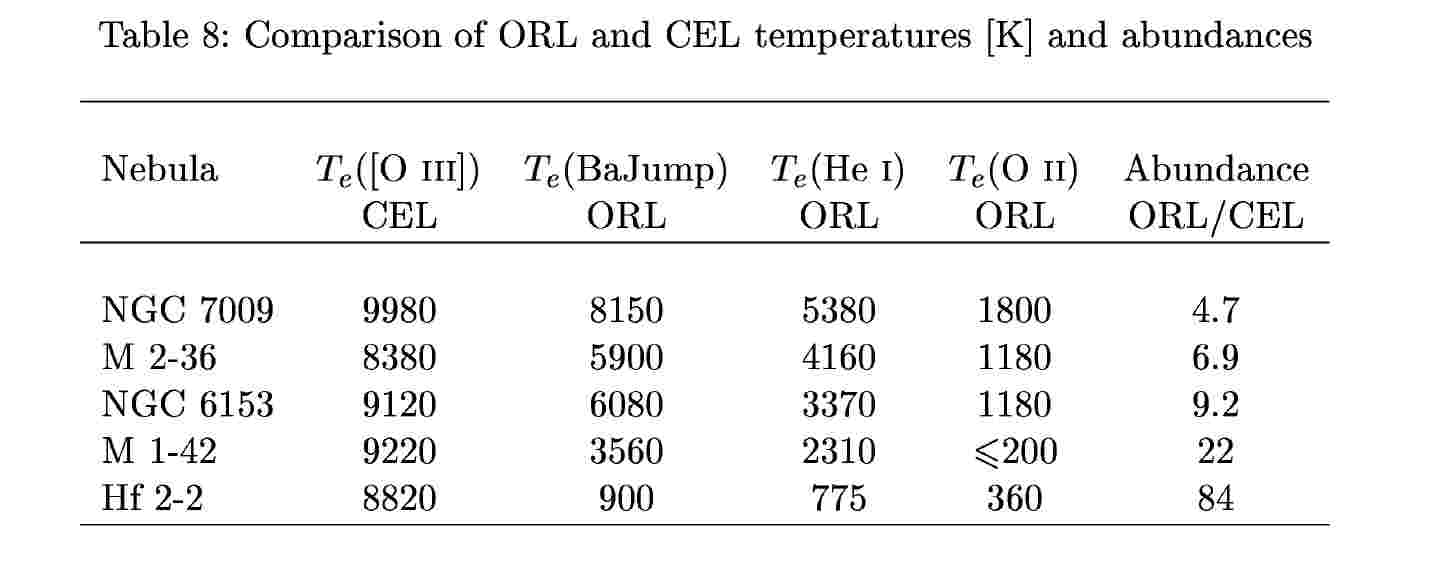
\includegraphics[width=\textwidth,height=!]{orl_cel_table.jpg}
\end{center}

\foilhead{\textcolor{red}{C$_5$} La discrepancia ORL/CEL -
soluci\'on?  }

Modelos de photoionisaci\'on con dos ``fases'' nebulares indican que
el grueso del material nebular ser\'{\i}a la componente caliente, el
que es trazado por las CELs (!' buena noticia!). \\

Un test para esta interpretaci\'on es estudiar el ensanchamiento
thermal de las l\'{\i}neas ORLs. 


